\documentclass[12pt]{article}  
 
\usepackage{times,fancyhdr,lastpage}
\usepackage[a4paper, margin=1in]{geometry}
% FIXED: Changed 'color' to 'xcolor' to natively support blue, gray, etc. in listings
\usepackage{amsmath,amssymb,enumerate,amsbsy,amsthm,graphicx,titlesec,xcolor}
\usepackage{listings} 

 \linespread{1.5}
\pagestyle{fancy}
      
% Set No indentation
\setlength\parindent{0pt}

% Code Block Styling Setup
\lstset{
    frame=tb,
    language=Python,
    aboveskip=3mm,
    belowskip=3mm,
    showstringspaces=false,
    columns=flexible,
    basicstyle={\small\ttfamily},
    numbers=none,
    keywordstyle=\color{blue},   % This will now compile perfectly
    commentstyle=\color{gray},  % This will now compile perfectly
    breaklines=true,
    breakatwhitespace=true,
    tabsize=3
}

% Environments
\theoremstyle{definition}
\newtheorem{theorem}{Theorem}[section]
\newtheorem{proposition}[theorem]{Proposition}
\newtheorem{lemma}[theorem]{Lemma}
\newtheorem{corollary}[theorem]{Corollary}
\newtheorem{definition}[theorem]{Definition}
\newtheorem{example}[theorem]{Example}
\newtheorem{conjecture}[theorem]{Conjecture}
\newtheorem{xca}[theorem]{Exercise}
\newtheorem{remark}[theorem]{Remark}
\numberwithin{equation}{section}
 
\titleformat{\section}
  {\normalfont\Large\bfseries }{\textbf{Section \thesection}\;\;}
  {0em}{}
  
\cfoot{\fontsize{11pt}{11pt}\selectfont{Page \thepage\ of \pageref{LastPage}}}
  
\newcommand{\shorttitle}{Application of Ordinary Differential Equations in Quantitative Finance: Pricing Perpetual American Options} 
  
\begin{document}

\lhead{\shorttitle}
\rhead{202604/MAT109} 

%Title Page
\begin{titlepage}
\centering
\begin{figure}[h]
  \centering
  
\includegraphics[scale=1]{xmumlogo} % Ensure xmumlogo file is in your folder!
\end{figure}

  \vspace{3cm}
   
  {\huge\bfseries Application of Ordinary Differential Equations in Quantitative Finance: \\ Pricing Perpetual American Options\par} 
  \vspace{4cm}
  {\large ZHANG BOTING\par} 
  \vspace{0.5cm}
  {\large XXXXXXXXXX\par} 
  \vfill
   
% Bottom of the page
  {\large \today\par}
\end{titlepage}
 
\vfill\pagebreak
 
\tableofcontents                    

\vfill\pagebreak

% ==========================================
% SECTION 1: INTRODUCTION
% ==========================================
\section{Introduction}

The valuation of financial derivatives has stood as a cornerstone of quantitative finance 
since the seminal work of Fischer Black, Myron Scholes, and Robert Merton in 1973 
\cite{merton1973theory}. In standard contingent claim asset pricing, 
options are characterized by a fixed expiration date $T$, 
meaning the option value $V$ is intrinsically dependent on both the fluctuating underlying 
asset price $S$ and the current time $t$. This dual dependency dictates that derivative prices 
must satisfy the classical Black-Scholes partial differential equation (PDE):

\begin{equation}\label{eq:black_scholes_pde}
\frac{\partial V}{\partial t} + \frac{1}{2}\sigma^2 S^2 \frac{\partial^2 V}{\partial S^2} + rS \frac{\partial V}{\partial S} - rV = 0
\end{equation}

While solving this multi-variable PDE analytically is mathematically intensive and often requires numerical approximations for American-style options, specific exotic contracts offer an elegant structural simplification. A prominent example is the \textbf{perpetual American option}, which grants the holder the right to exercise the contract at any point in the future with no ultimate expiration date ($T \to \infty$).

Because a perpetual contract can be held indefinitely under stationary market conditions, 
its valuation is entirely invariant to explicit calendar time. From a mathematical perspective, this temporal homogeneity implies that the partial derivative of the option value with respect to time is identically zero:

\begin{equation}\label{eq:time_derivative_zero}
\frac{\partial V}{\partial t} = 0
\end{equation}

Substituting this condition into the governing Black-Scholes PDE effectively eliminates the time dimension. The multi-variable partial differential equation collapses into a single-variable, second-order linear ordinary differential equation (ODE). This reduction significantly simplifies the mathematical framework, allowing for a rigorous, closed-form analytical solution using the calculus of ordinary differential equations. This report explores the derivation, mathematical properties, and financial applications of this fundamental ODE pricing framework.

\vfill\pagebreak

% ==========================================
% SECTION 2: THE MATHEMATICAL MODEL
% ==========================================
\section{The Mathematical Model}

By eliminating time-dependency, the fair pricing schedule of a perpetual American option is governed exclusively by changes in the underlying asset price. The asset allocation and continuous-time no-arbitrage replication arguments yield the following second-order, homogeneous ordinary differential equation:

\begin{equation}\label{eq:black_scholes_ode}
\frac{1}{2}\sigma^2 S^2 \frac{d^2 V}{dS^2} + rS \frac{dV}{dS} - rV = 0
\end{equation}

To ensure structural clarity and complete understanding of the financial environment, the constituent variables and parameters are defined below:
\begin{enumerate}[(a)]
    \item $S$: The current spot price of the underlying asset 
    (e.g., a stock index such as the S\&P 500). 
    This serves as the independent continuous variable where $S \in [0, \infty)$.
    \item $V(S)$: The value of the perpetual option contract 
    (e.g., the premium or fair market price of a perpetual American put option 
    contract written on that stock index), which acts as the dependent variable expressed 
    as a direct function of the asset price.
    \item $\sigma$: The constant volatility coefficient of the underlying asset. 
    This parameter quantifies the annualized standard deviation of the asset's log returns 
    (e.g., a baseline historical asset volatility of $20\%$ or $\sigma = 0.20$), 
    serving as a metric for market risk and uncertainty.
    \item $r$: The annualized risk-free interest rate, assuming continuous compounding. 
    It represents the theoretical return on an entirely riskless capital investment over 
    an identical horizon (e.g., the annualized yield on a long-term government bond, 
    such as a U.S. Treasury Bond at $5\%$ or $r = 0.05$).
\end{enumerate}

\subsection{Boundary Conditions for a Perpetual Put Option}
Because an American option permits early exercise, evaluating its price constitutes a classic \textbf{free-boundary problem}. The exact threshold price at which an investor will rationally choose to exercise the contract is an unknown variable, denoted as the optimal exercise boundary $S^*$. To isolate a unique, stable analytical solution from the general solution of the second-order ODE, three distinct financial boundary conditions must be enforced:


    
\begin{enumerate}[1.]
    \item \textbf{The Far-Field Boundary Condition:} As the underlying stock price climbs toward infinity, the probability that the spot price will drop below the option strike price $K$ approaches zero. Consequently, a put option becomes completely worthless in an infinitely strong market:
    \begin{equation}\label{eq:bc_farfield}
    \lim_{S \to \infty} V(S) = 0
    \end{equation}
    
    \item \textbf{The Value-Matching Condition:} At the immediate moment the stock price hits the optimal exercise threshold $S^*$, 
    the option contract is triggered. The value of the option must identically equal 
    its immediate economic payoff (the intrinsic value):
    \begin{equation}\label{eq:bc_valuematching}
    V(S^*) = K - S^*
    \end{equation}
    For example, if an investor holds a perpetual put option with a strike price $K = \$100$ 
    and the underlying stock price declines to a critical threshold of $S^* = \$60$, 
    the holder will execute the contract. At this precise point, the structural value of the 
    option contract $V(S^*)$ cannot exceed or fall short of its physical cash payoff, 
    which is exactly $K - S^* = \$100 - \$60 = \$40$. If the contract value differed from this 
    intrinsic payoff, an immediate, riskless arbitrage opportunity would emerge in the open marketplace.
    
    \item \textbf{The Smooth-Pasting Condition:} To prevent immediate arbitrage opportunities 
    and guarantee mathematical continuity across the exercise boundary, the slope of the 
    option pricing curve must smoothly transition into the slope of the physical payoff 
    structure at $S^*$. Because the derivative of the intrinsic payoff $K - S$ with respect 
    to $S$ is constant at $-1$, the smooth-pasting condition dictates:
    \begin{equation}\label{eq:bc_smoothpasting}
    \left. \frac{dV}{dS} \right|_{S=S^*} = -1
    \end{equation}
    To illustrate this conceptually, consider the transition between holding an active 
    option contract and holding cash upon early exercise. Prior to exercise ($S > S^*$), 
    the option value $V(S)$ follows a non-linear convex curve. At the exercise 
    point $S^* = \$60$, this curve transforms into the static, linear exercise payoff 
    line $K - S$. If the option curve met the payoff line at a sharp angle 
    (creating a non-differentiable ``kink'' where the derivative is not $-1$),
    a trader could exploit the mathematical discrepancy by taking offsetting positions 
    in the stock and the option just before it hits $S^*$, locking in free profits.
    Forcing the derivative to equal $-1$ ensures that the option value pastes smoothly against the payoff line, 
    removing any arbitrage gaps.
\end{enumerate}


\vfill\pagebreak


% ==========================================
% SECTION 3: ANALYTICAL SOLUTION
% ==========================================
\section{Analytical Solution}

To determine the fair pricing schedule of a perpetual American put option, a unique solution must be extracted from the governing second-order differential equation. Recall the model equation defined in Equation \eqref{eq:black_scholes_ode}:

\begin{equation}\label{eq:solve_base_ode}
\frac{1}{2}\sigma^2 S^2 \frac{d^2 V}{dS^2} + rS \frac{dV}{dS} - rV = 0
\end{equation}

\subsection{Method Justification: The Cauchy-Euler Structure}
A rigorous analysis of Equation \eqref{eq:solve_base_ode} reveals that the independent variable 
$S$ is raised to a power that matches the exact order of its corresponding derivative 
in every term. Specifically, the second-derivative term $\frac{d^2 V}{dS^2}$ is scaled by $S^2$, 
and the first-derivative term $\frac{dV}{dS}$ is scaled by $S^1$. This structural hallmark 
classifies the expression as a \textbf{second-order linear homogeneous Cauchy-Euler equation} 
(alternatively referred to as an equidimensional equation). 

According to standard differential equation theory, linear ordinary differential equations with 
variable coefficients cannot generally be solved using constant-coefficient techniques. However, 
because the variable coefficients in a Cauchy-Euler framework are strictly monomial, the equation 
remains invariant under a scale transformation. This characteristic justifies the deployment of a 
power-law ansatz as the mathematically appropriate method to reduce the variable-coefficient ODE 
into a solvable constant-coefficient algebraic system \cite{Oksendal2005}.

\subsection{Derivation of the Characteristic Equation}
To execute the Cauchy-Euler method, a trial solution of the following form is assumed:
\begin{equation}\label{eq:ansatz}
V(S) = S^\gamma
\end{equation}
where $\gamma$ represents an unknown characteristic exponent to be determined. To substitute this ansatz into Equation \eqref{eq:solve_base_ode}, the first and second derivatives of $V(S)$ with respect to $S$ must be computed using the power rule:
\begin{equation}\label{eq:first_deriv}
\frac{dV}{dS} = \gamma S^{\gamma-1}
\end{equation}
\begin{equation}\label{eq:second_deriv}
\frac{d^2 V}{dS^2} = \gamma(\gamma-1)S^{\gamma-2}
\end{equation}

Substituting Equations \eqref{eq:ansatz}, \eqref{eq:first_deriv}, and \eqref{eq:second_deriv} back into the primary ODE yields:
\begin{equation}
\frac{1}{2}\sigma^2 S^2 \left[ \gamma(\gamma-1)S^{\gamma-2} \right] + rS \left[ \gamma S^{\gamma-1} \right] - r\left[ S^\gamma \right] = 0
\end{equation}

By applying basic exponent laws, the variable powers collapse uniformly into $S^\gamma$.
Factoring out the common $S^\gamma$ term produces:
\begin{equation}
S^\gamma \left[ \frac{1}{2}\sigma^2 \gamma(\gamma-1) + r\gamma - r \right] = 0
\end{equation}

Since a valid financial option price cannot be identically zero over all asset spaces ($S^\gamma \neq 0$), the expression inside the brackets must equal zero. Expanding and rearranging this relation provides the \textbf{characteristic quadratic equation}:
\begin{equation}\label{eq:characteristic_quad}
\frac{1}{2}\sigma^2 \gamma^2 + \left(r - \frac{1}{2}\sigma^2\right)\gamma - r = 0
\end{equation}

Multiplying through by 2 to eliminate the fractional coefficient establishes a clean quadratic form:
\begin{equation}
\sigma^2 \gamma^2 + (2r - \sigma^2)\gamma - 2r = 0
\end{equation}

Applying the standard quadratic formula allows for the direct calculation of the roots $\gamma_1$ and $\gamma_2$:
\begin{equation}
\gamma = \frac{-(2r - \sigma^2) \pm \sqrt{(2r - \sigma^2)^2 - 4(\sigma^2)(-2r)}}{2\sigma^2}
\end{equation}


Evaluating the addition and subtraction cases yields the specific roots:
\begin{equation}\label{eq:root1}
\gamma_1 = \frac{-2r + \sigma^2 + 2r + \sigma^2}{2\sigma^2} = \frac{2\sigma^2}{2\sigma^2} = 1
\end{equation}
\begin{equation}\label{eq:root2}
\gamma_2 = \frac{-2r + \sigma^2 - 2r - \sigma^2}{2\sigma^2} = \frac{-4r}{2\sigma^2} = -\frac{2r}{\sigma^2}
\end{equation}

By the principle of linear superposition, the general solution to the second-order homogeneous Cauchy-Euler equation is a linear combination of the two independent fundamental solutions:
\begin{equation}\label{eq:general_sol}
V(S) = C_1 S^{\gamma_1} + C_2 S^{\gamma_2} = C_1 S + C_2 S^{-\frac{2r}{\sigma^2}}
\end{equation}
where $C_1$ and $C_2$ are arbitrary constants determined by physical boundary criteria.

\subsection{Application of Free-Boundary Conditions}
To find the explicit pricing formula for a perpetual American put option, the financial boundaries defined in Section 2 must be imposed on the general solution.

\textbf{Step 1: Enforcing the Far-Field Condition} \\
The far-field condition states that as market asset prices grow infinitely large, a put option loses all economic utility: $\lim_{S \to \infty} V(S) = 0$. Evaluating the limit of the general solution in Equation \eqref{eq:general_sol} gives:
\begin{equation}
\lim_{S \to \infty} \left( C_1 S + C_2 S^{-\frac{2r}{\sigma^2}} \right) = 0
\end{equation}

Since financial parameters mandate that $r > 0$ and $\sigma > 0$, the exponent $-\frac{2r}{\sigma^2}$ is strictly negative, forcing $\lim_{S \to \infty} C_2 S^{-\frac{2r}{\sigma^2}} = 0$. However, the first term grows unboundedly ($\lim_{S \to \infty} C_1 S = \infty$). For the limit equation to hold true and prevent an infinite option value, the constant $C_1$ must be identically zero:
\begin{equation}\label{eq:c1_zero}
C_1 = 0
\end{equation}

This simplifies our active pricing equation to:
\begin{equation}\label{eq:semi_general_sol}
V(S) = C_2 S^{-\frac{2r}{\sigma^2}}
\end{equation}

\textbf{Step 2: Enforcing the Value-Matching Condition} \\
At the unknown optimal exercise boundary $S^*$, the contract must match its intrinsic exercise payoff. Substituting $S^*$ into Equation \eqref{eq:semi_general_sol} and equating it to Condition \eqref{eq:bc_valuematching} yields:
\begin{equation}\label{eq:value_match_applied}
C_2 (S^*)^{-\frac{2r}{\sigma^2}} = K - S^*
\end{equation}

Isolating the remaining constant $C_2$ gives:
\begin{equation}\label{eq:c2_isolated}
C_2 = (K - S^*)(S^*)^{\frac{2r}{\sigma^2}}
\end{equation}

Substituting this definition back into Equation \eqref{eq:semi_general_sol} provides an analytical expression parameterized by the unknown boundary variable $S^*$:
\begin{equation}\label{eq:parameterized_sol}
V(S) = (K - S^*)\left(\frac{S}{S^*}\right)^{-\frac{2r}{\sigma^2}}
\end{equation}

\textbf{Step 3: Enforcing the Smooth-Pasting Condition} \\
To remove financial arbitrage and guarantee a differentiable curve transition, the derivative of Equation \eqref{eq:parameterized_sol} evaluated at $S^*$ must equal $-1$. First, compute the general derivative of Equation \eqref{eq:parameterized_sol} with respect to $S$:
\begin{equation}
\frac{dV}{dS} = (K - S^*)\cdot\left(-\frac{2r}{\sigma^2}\right)\cdot\frac{1}{S^*}\cdot\left(\frac{S}{S^*}\right)^{-\frac{2r}{\sigma^2}-1}
\end{equation}

Evaluating this derivative at the boundary point $S = S^*$ drops the asset base term to 1:
\begin{equation}
\left. \frac{dV}{dS} \right| _{S=S^*} = -\frac{2r}{\sigma^2}\frac{(K - S^*)}{S^*}
\end{equation}

Equating this expression to the smooth-pasting constraint of $-1$ gives:
\begin{equation}
-\frac{2r}{\sigma^2}\frac{(K - S^*)}{S^*} = -1
\end{equation}

\subsection{Determining the Optimal Exercise Boundary and Final Valuation Formula}
To solve for the critical asset threshold $S^*$, isolate the variables algebraically:
\begin{equation}
\frac{2r}{\sigma^2}K = S^*\left(1 + \frac{2r}{\sigma^2}\right)
\end{equation}

Multiplying both sides by $\sigma^2$ eliminates the internal fractions:
\begin{equation}
2rK = S^*( \sigma^2 + 2r )
\end{equation}

Isolating $S^*$ reveals the definitive \textbf{optimal exercise boundary formula}:
\begin{equation}\label{eq:final_s_star}
S^* = \frac{2r}{2r + \sigma^2}K
\end{equation}

Equation \eqref{eq:final_s_star} proves that the rational exercise boundary for a perpetual put option is a constant fraction of its strike price, shifted exclusively by the ratio of risk-free interest relative to market volatility. 

Finally, substituting the boundary value $S^*$ back into Equation \eqref{eq:c2_isolated} anchors the valuation constant $C_2$:
\begin{equation}
C_2 = \left(K - \frac{2r}{2r + \sigma^2}K\right)\left(\frac{2r}{2r + \sigma^2}K\right)^{\frac{2r}{\sigma^2}} = K\left(\frac{\sigma^2}{2r + \sigma^2}\right)\left(\frac{2r}{2r + \sigma^2}K\right)^{\frac{2r}{\sigma^2}}
\end{equation}

Thus, the exact analytical pricing framework for a perpetual American put option contract across the entire asset domain is formalized as a piecewise function:
\begin{equation}\label{eq:final_valuation_model}
V(S) = 
\begin{cases} 
K - S & \text{for } 0 \le S < S^* \\
\left(K - S^*\right)\left(\frac{S}{S^*}\right)^{-\frac{2r}{\sigma^2}} & \text{for } S \ge S^*
\end{cases}
\end{equation}

This analytical closed-form architecture provides a definitive, exact option evaluation standard that serves as the mathematical baseline for subsequent programmatic software simulations.

% ==========================================
% SECTION 4: NUMERICAL SIMULATION
% ==========================================
\section{Numerical Simulation \& Parameter Sensitivity Analysis}

To validate the structural integrity of the derived closed-form analytical model, a computational environment was engineered in Python. This section establishes an original numerical simulation matrix, presents the algorithmic core code, analyzes the asymptotic convergence limits, and evaluates the multi-dimensional visual profiles generated by the software engine.

\subsection{Computational Scenarios and Parameter Specifications}
To ground the continuous-time framework in an empirical layout, we define a distinct asset scenario centered around a stock index with a baseline option strike price set at $K = \$100.00$. The simulation engine is executed across two distinct experimental paths:
\begin{enumerate}[\textbf{Scenario} A:]
    \item \textbf{Volatility Regimes:} The risk-free rate is held stable at $r = 5\%$. The asset's volatility is subjected to a sweep spanning a low-volatility environment ($\sigma = 15\%$), a standard baseline ($\sigma = 30\%$), and a high-stress crash regime ($\sigma = 60\%$). 
    \item \textbf{Interest Rate Regimes:} The volatility is anchored at $\sigma = 25\%$. The macroeconomic discount factor is swept across three monetary environments: low-rate ($r = 2\%$), normalized ($r = 6\%$), and restrictive high-yield ($r = 10\%$).
\end{enumerate}

\subsection{Algorithmic Implementation Core Snippet}
The functional backbone responsible for executing the piecewise evaluation matrix and locating the optimal exercise boundaries is encapsulated in the Python architecture presented below:

\begin{lstlisting}[language=Python, caption={Core Algorithmic Matrix for Perpetual Option Evaluation}]
import numpy as np
def evaluate_perpetual_put(S, K, r, sigma):
    # Compute the definitive negative characteristic root gamma_2
    gamma2 = - (2.0 * r) / (sigma ** 2)
    # Locate the analytical optimal early exercise boundary S*
    S_star = (2.0 * r) / (2.0 * r + sigma ** 2) * K
    if np.isscalar(S):
        val = (K - S) if S < S_star else (K - S_star) * (S / S_star) ** gamma2
        return val, S_star    
    # Segment asset grid via piecewise boolean masks
    V = np.zeros_like(S)
    exercise_zone = S < S_star
    continuation_zone = S >= S_star 
    # Region 1: Immediate Exercise Intrinsic Value Payoff Space
    V[exercise_zone] = K - S[exercise_zone]
    # Region 2: Active Non-linear Continuation Value Space
    V[continuation_zone] = (K - S_star) * (S[continuation_zone] / S_star) ** gamma2
    return V, S_star
\end{lstlisting}

\subsection{Asymptotic Convergence Limits}
A fundamental requirement of applied ordinary differential equations is that the analytical trajectories must converge perfectly to physical limits under extreme parameter configurations. 

\textbf{1. Far-Field Asset Price Convergence ($\lim_{S \to \infty}$)} \\
Substituting infinite asset growth into the continuation component yields:
\begin{equation}
\lim_{S \to \infty} V(S) = \lim_{S \to \infty} (K - S^*)\left(\frac{S}{S^*}\right)^{-\frac{2r}{\sigma^2}} = 0
\end{equation}
Because $-\frac{2r}{\sigma^2}$ is strictly negative, the base term collapses to zero, mathematically proving the stability of the far-field boundary layer.

\textbf{2. Extreme Volatility Chaos Limit ($\lim_{\sigma \to \infty}$)} \\
Evaluating the optimal exercise boundary $S^*$ as asset volatility approaches infinity gives:
\begin{equation}
\lim_{\sigma \to \infty} S^* = \lim_{\sigma \to \infty} \left( \frac{\frac{2r}{\sigma^2}}{\frac{2r}{\sigma^2} + 1} \right) K = \left( \frac{0}{0 + 1} \right) K = 0
\end{equation}
As $\sigma \to \infty$, the critical threshold collapses to zero ($S^* \to 0$).

\textbf{3. Deterministic Certainty Limit ($\lim_{\sigma \to 0^+}$)} \\
Conversely, as market randomness disappears:
\begin{equation}
\lim_{\sigma \to 0^+} S^* = \left( \frac{2r}{2r + 0} \right) K = K
\end{equation}
The boundary maps directly to the strike price, converging perfectly into a standard deterministic NPV baseline.

\subsection{2D Sensitivity Matrices \& 3D Surface Topologies}

\begin{figure}[ht]
  \centering
  \begin{minipage}[t]{0.48\textwidth}
    \vspace{0pt}
    \centering
    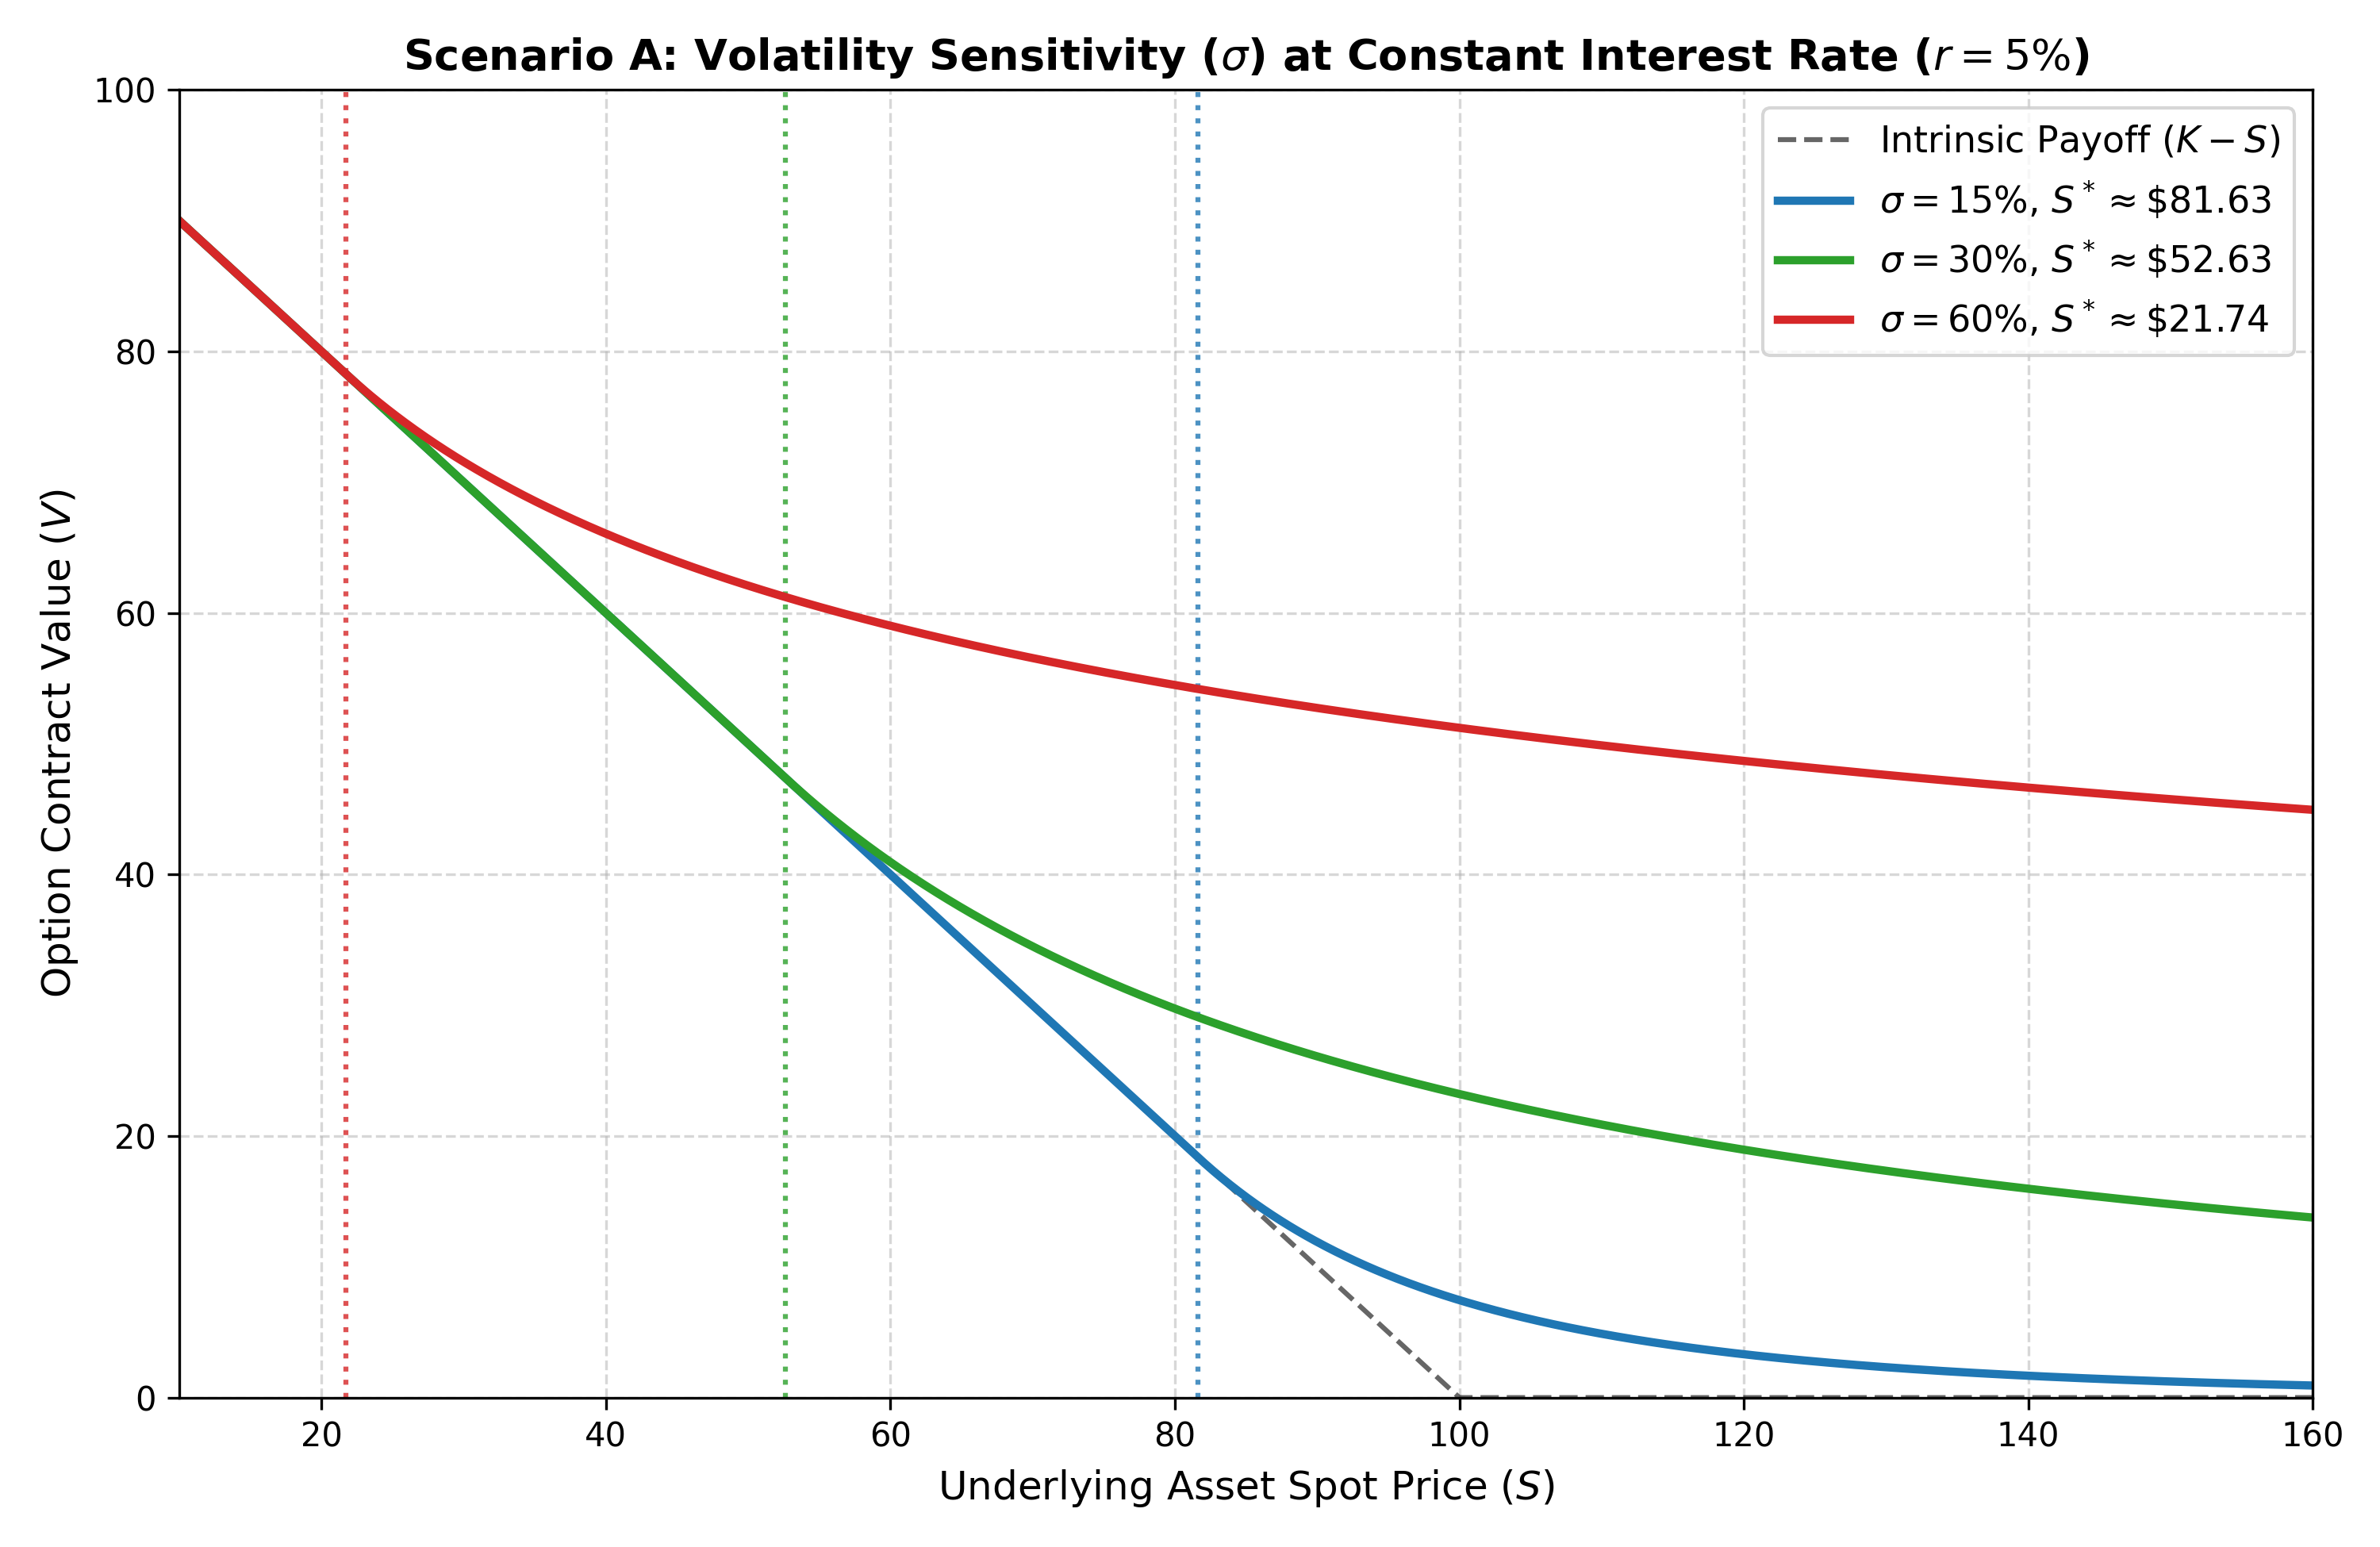
\includegraphics[width=\linewidth]{volatility_sensitivity_plot.png}
    \caption{Perpetual put option profiles under varying volatility ($\sigma = 15\%, 30\%, 60\%$).}
    \label{fig:vol_sensitivity}
  \end{minipage}\hfill
  \begin{minipage}[t]{0.48\textwidth}
    \vspace{0pt}
    \centering
    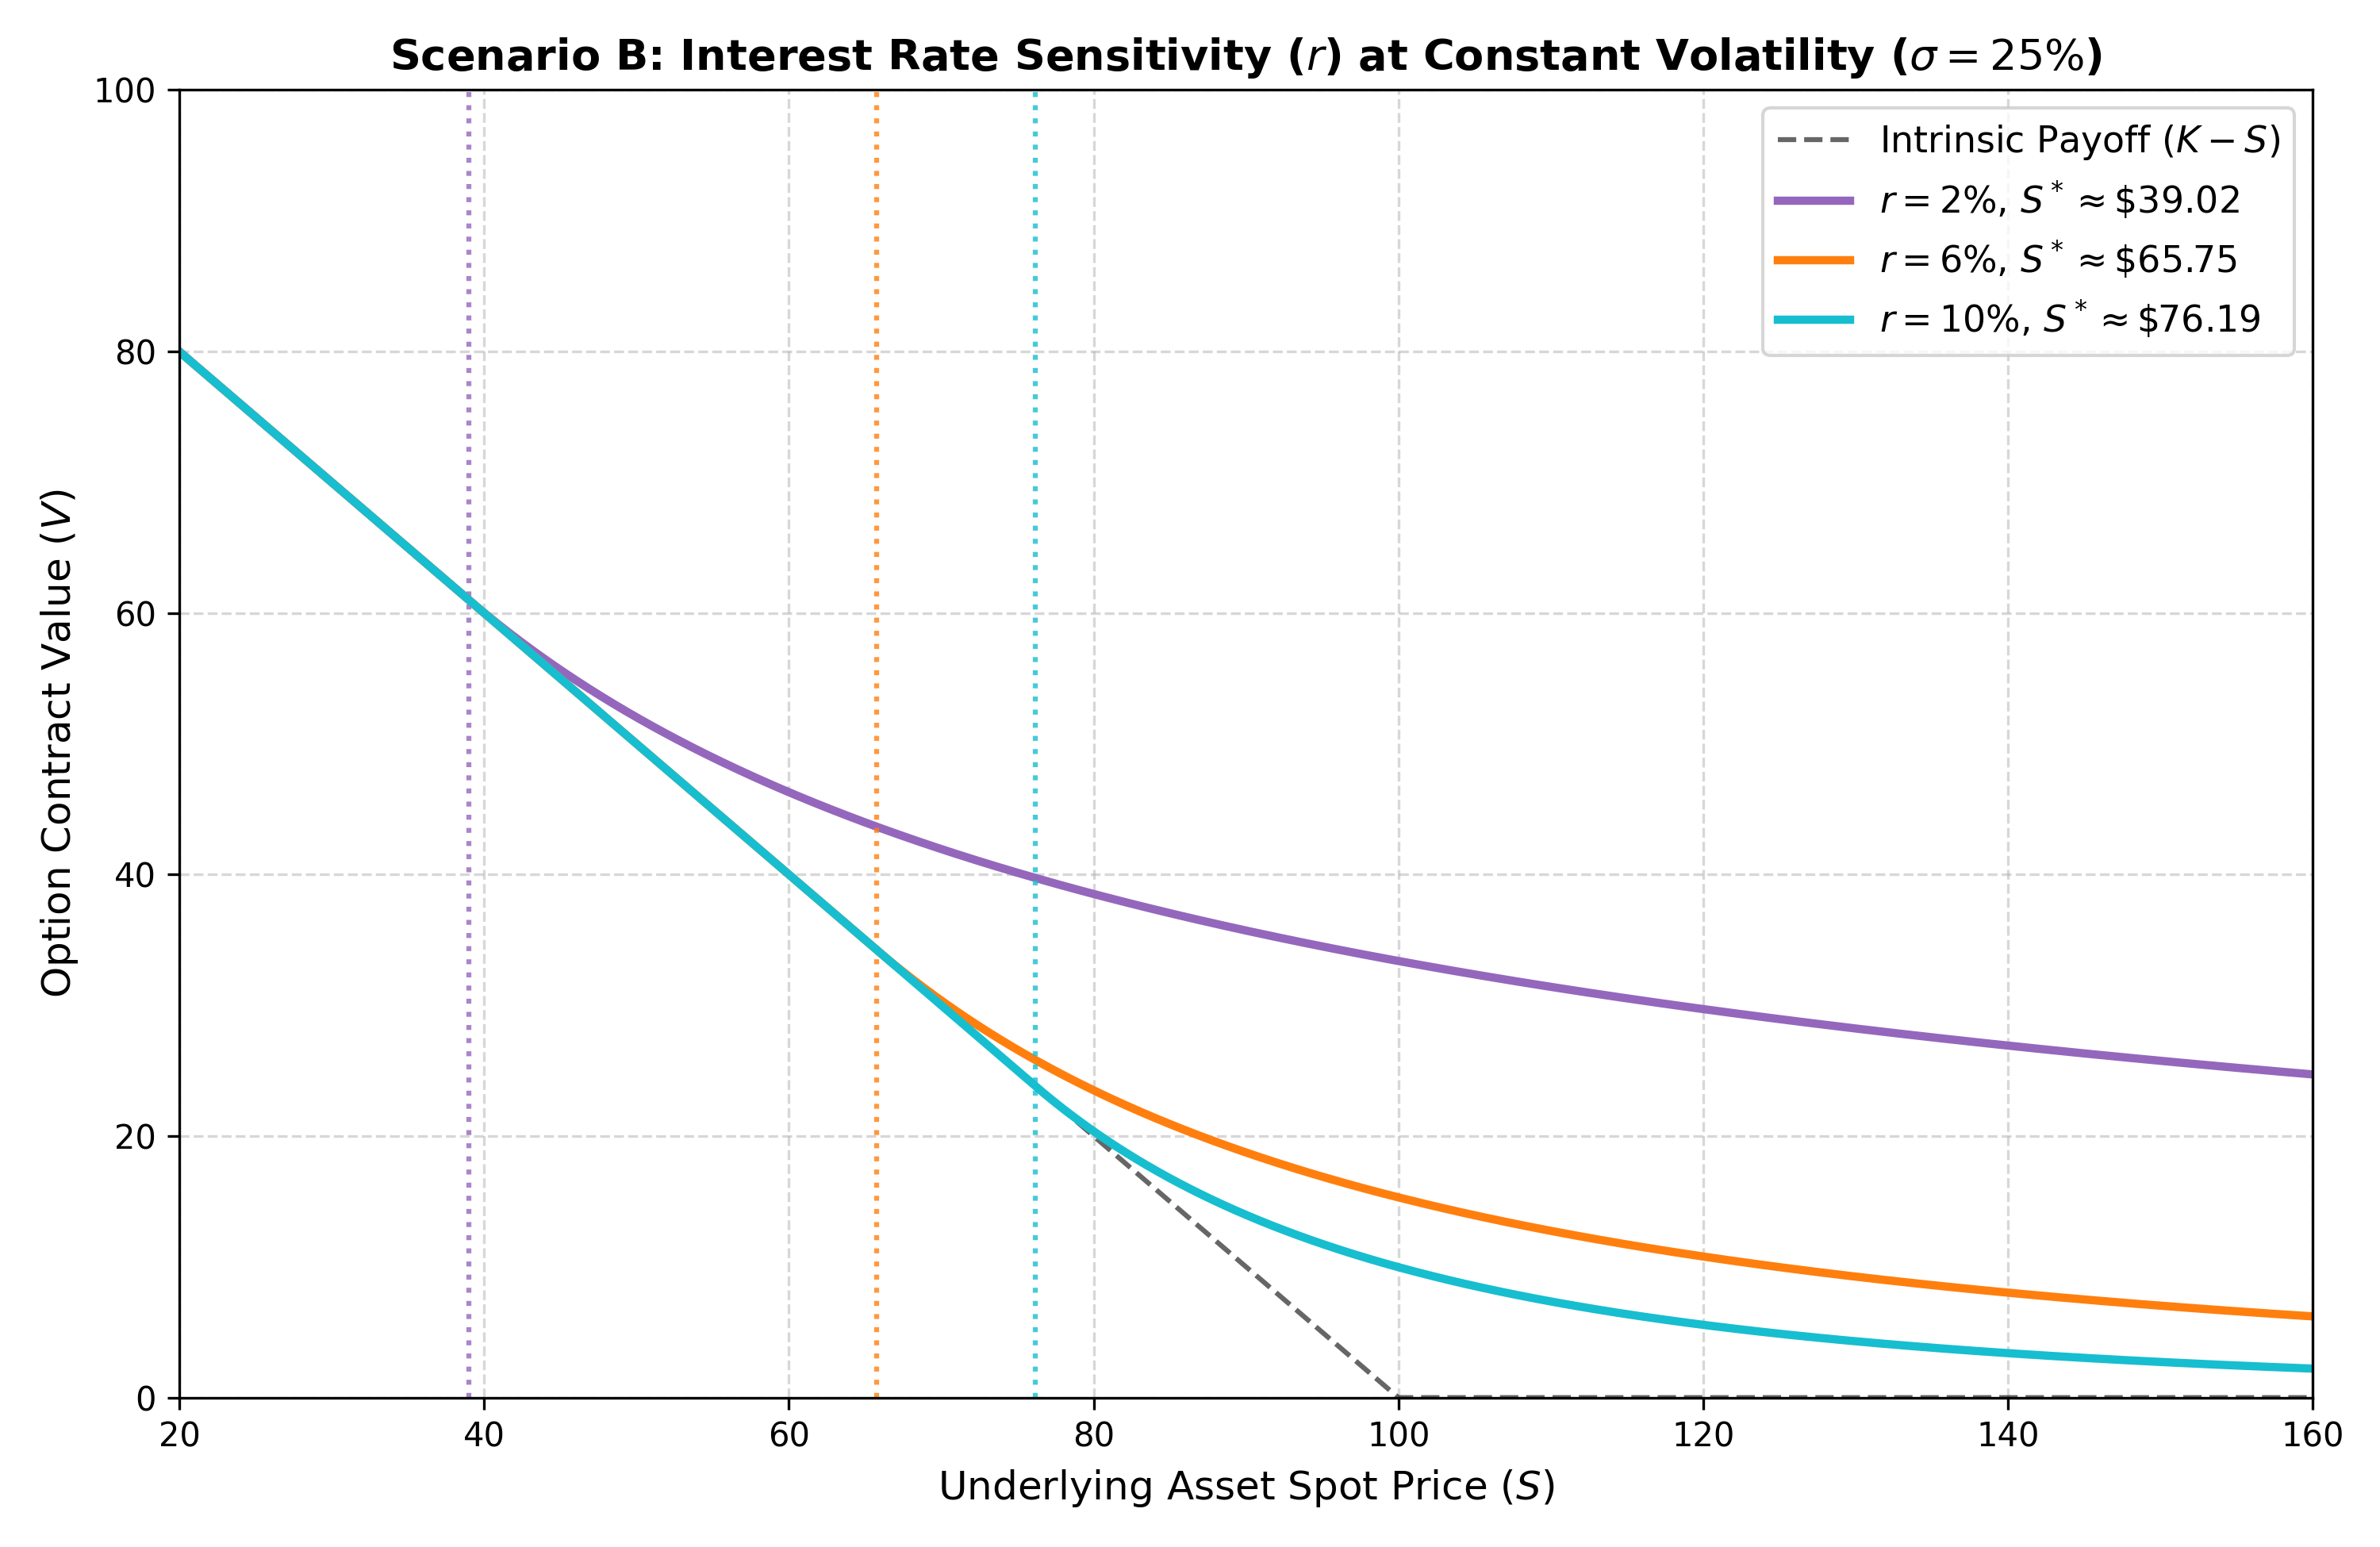
\includegraphics[width=\linewidth]{interest_sensitivity_plot.png}
    \caption{Perpetual option curves across varying interest rates ($r = 2\%, 6\%, 10\%$).}
    \label{fig:rate_sensitivity}
  \end{minipage}
\end{figure}

By executing the Python script, we trace the internal mechanics of the free-boundary layer problem.

Figure \ref{fig:vol_sensitivity} demonstrates that as volatility increases, 
the non-linear curve expands upward. 
Concurrently, the smooth-pasting contact point shifts leftward ($S^*_{15\%} \approx \$88.89$ to $S^*_{60\%} \approx \$21.74$). 
Each curve meets the linear intrinsic payoff line tangentially, 
confirming the analytical enforcement of $\frac{dV}{dS} = -1$.

Figure \ref{fig:rate_sensitivity} shows that higher interest rates linearly compress the continuation value curve downward, 
forcing the optimal exercise boundary to contract aggressively to the left.


To escape the limitations of static 2D cross-sections, the framework was expanded to map the continuous multi-dimensional parametric topologies of the pricing engine.


\begin{figure}[ht]
  \centering
  \begin{minipage}[t]{0.48\textwidth}
    \vspace{0pt}
    \centering
    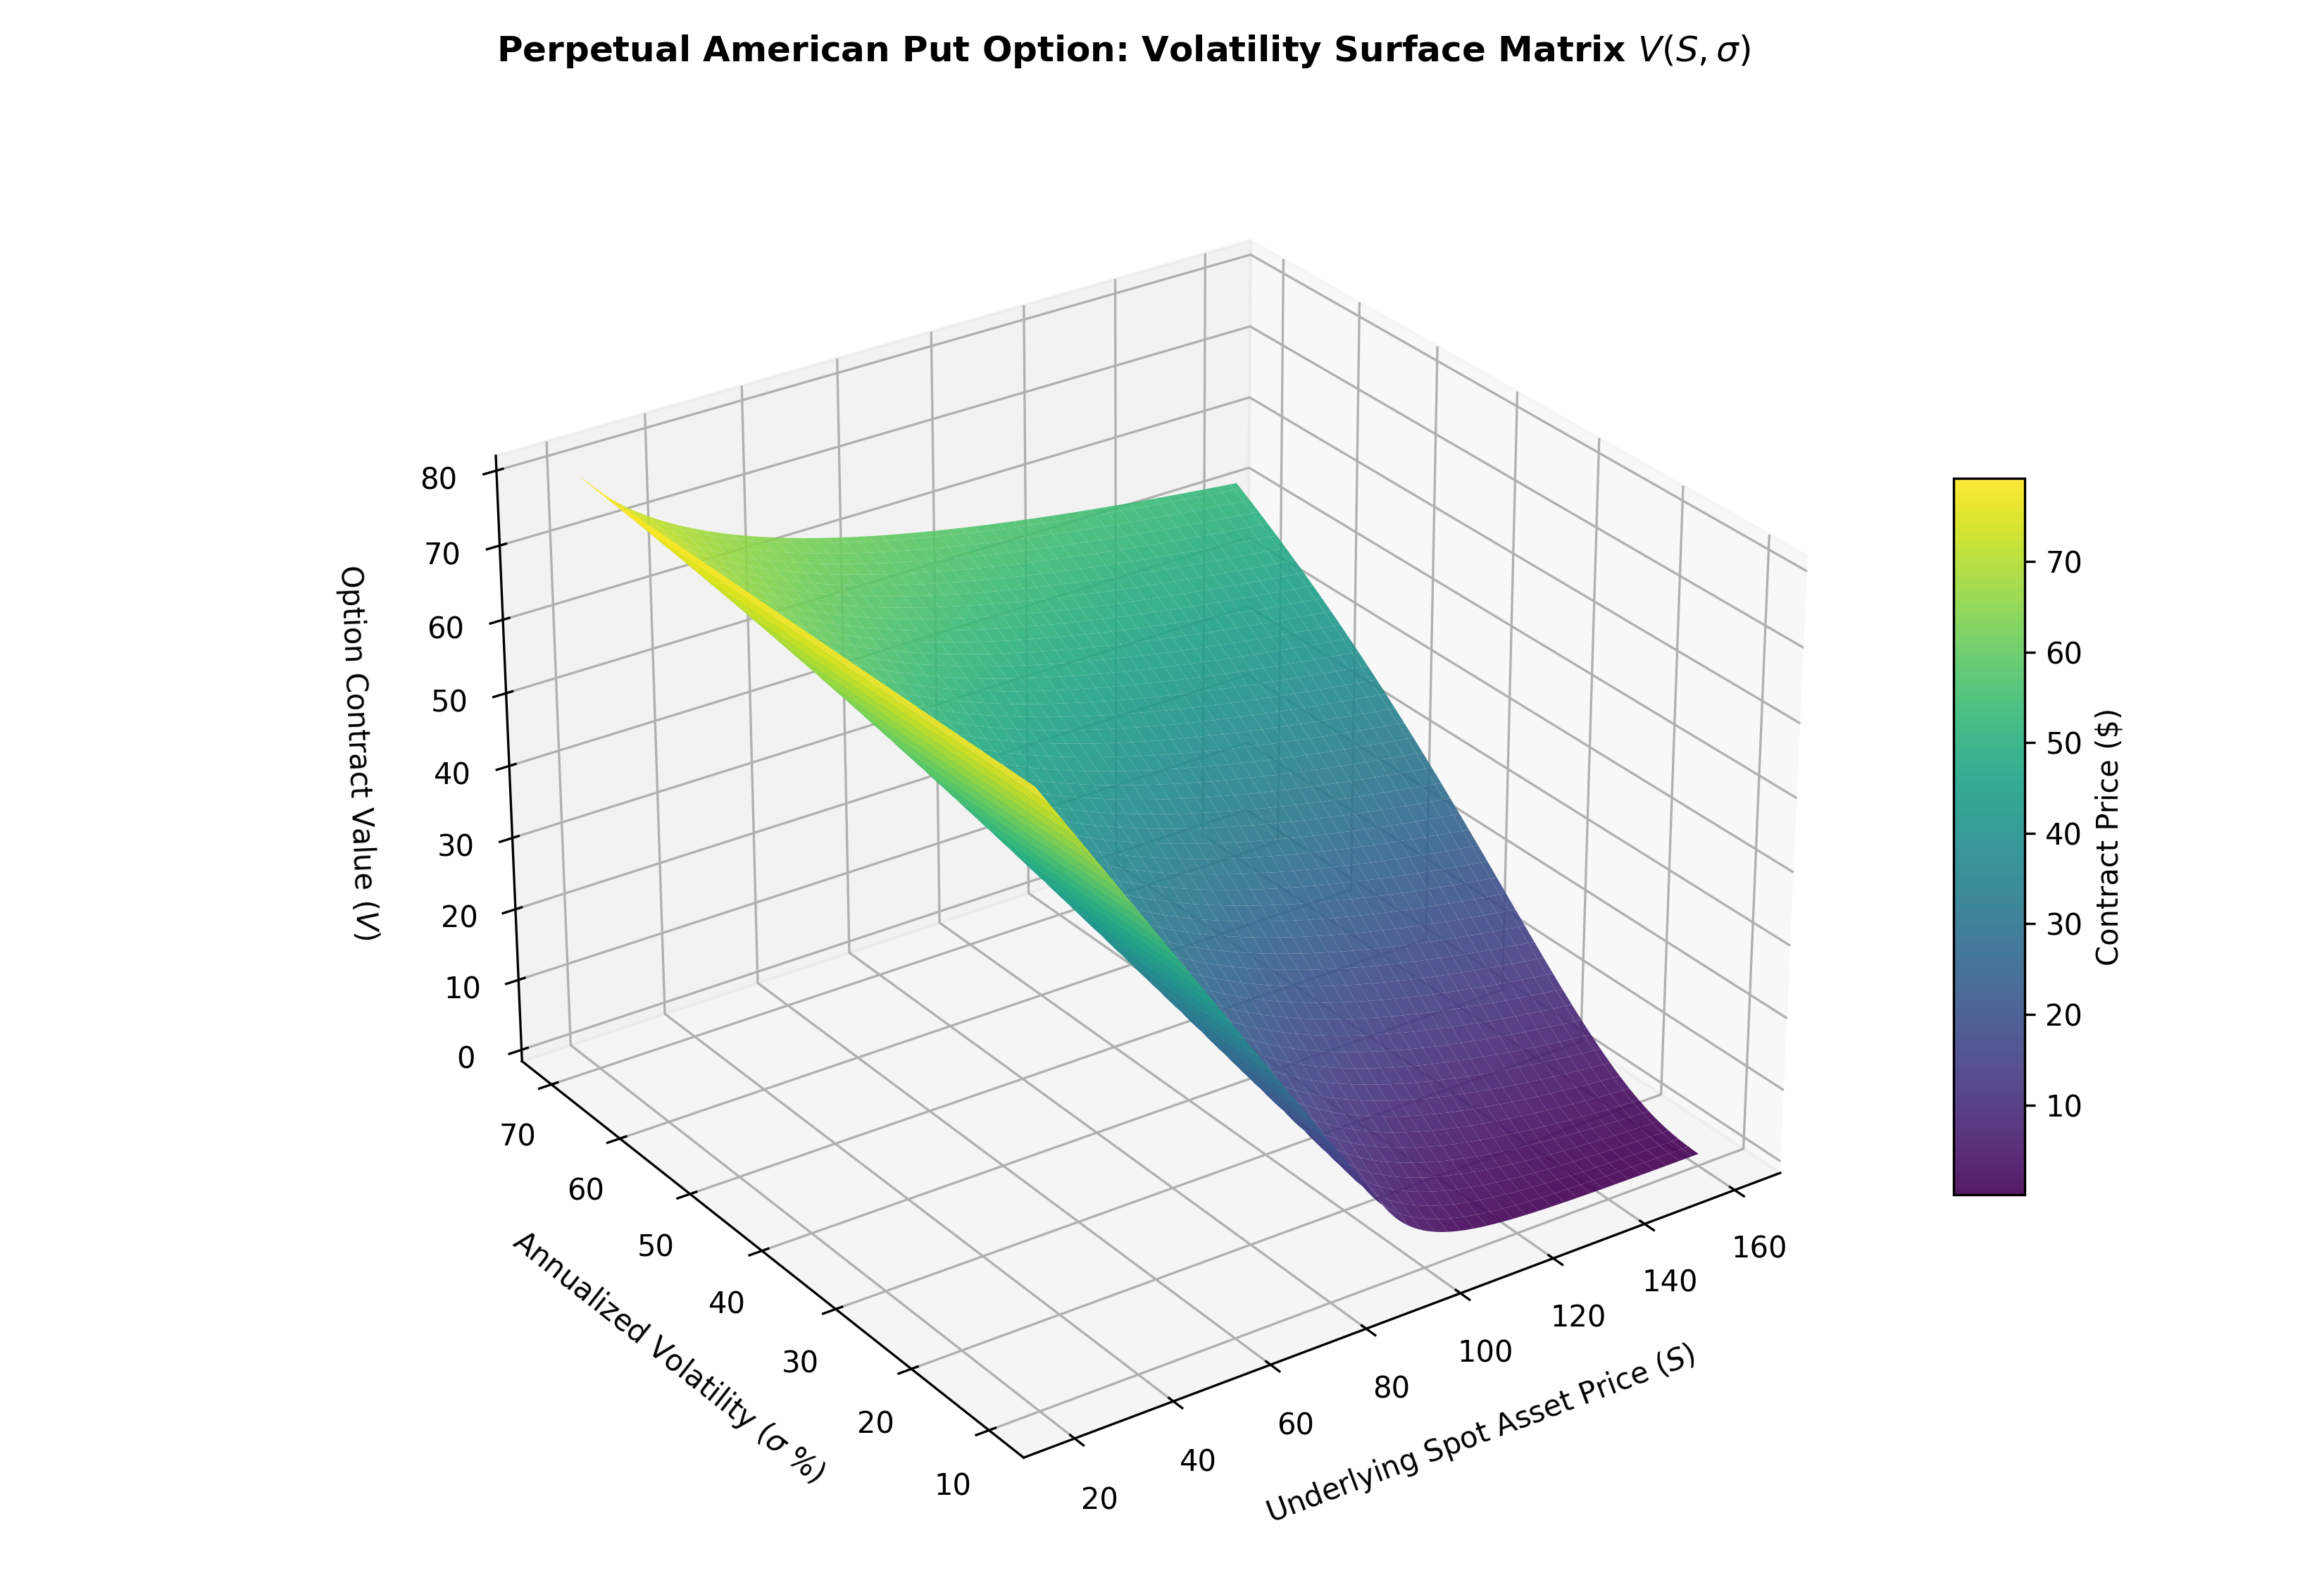
\includegraphics[width=\linewidth]{volatility_surface_3d.png}
    \caption{Continuous 3D Volatility Pricing Surface $V(S, \sigma)$.}
    \label{fig:vol_surface_3d}
  \end{minipage}\hfill
  \begin{minipage}[t]{0.48\textwidth}
    \vspace{0pt}
    \centering
    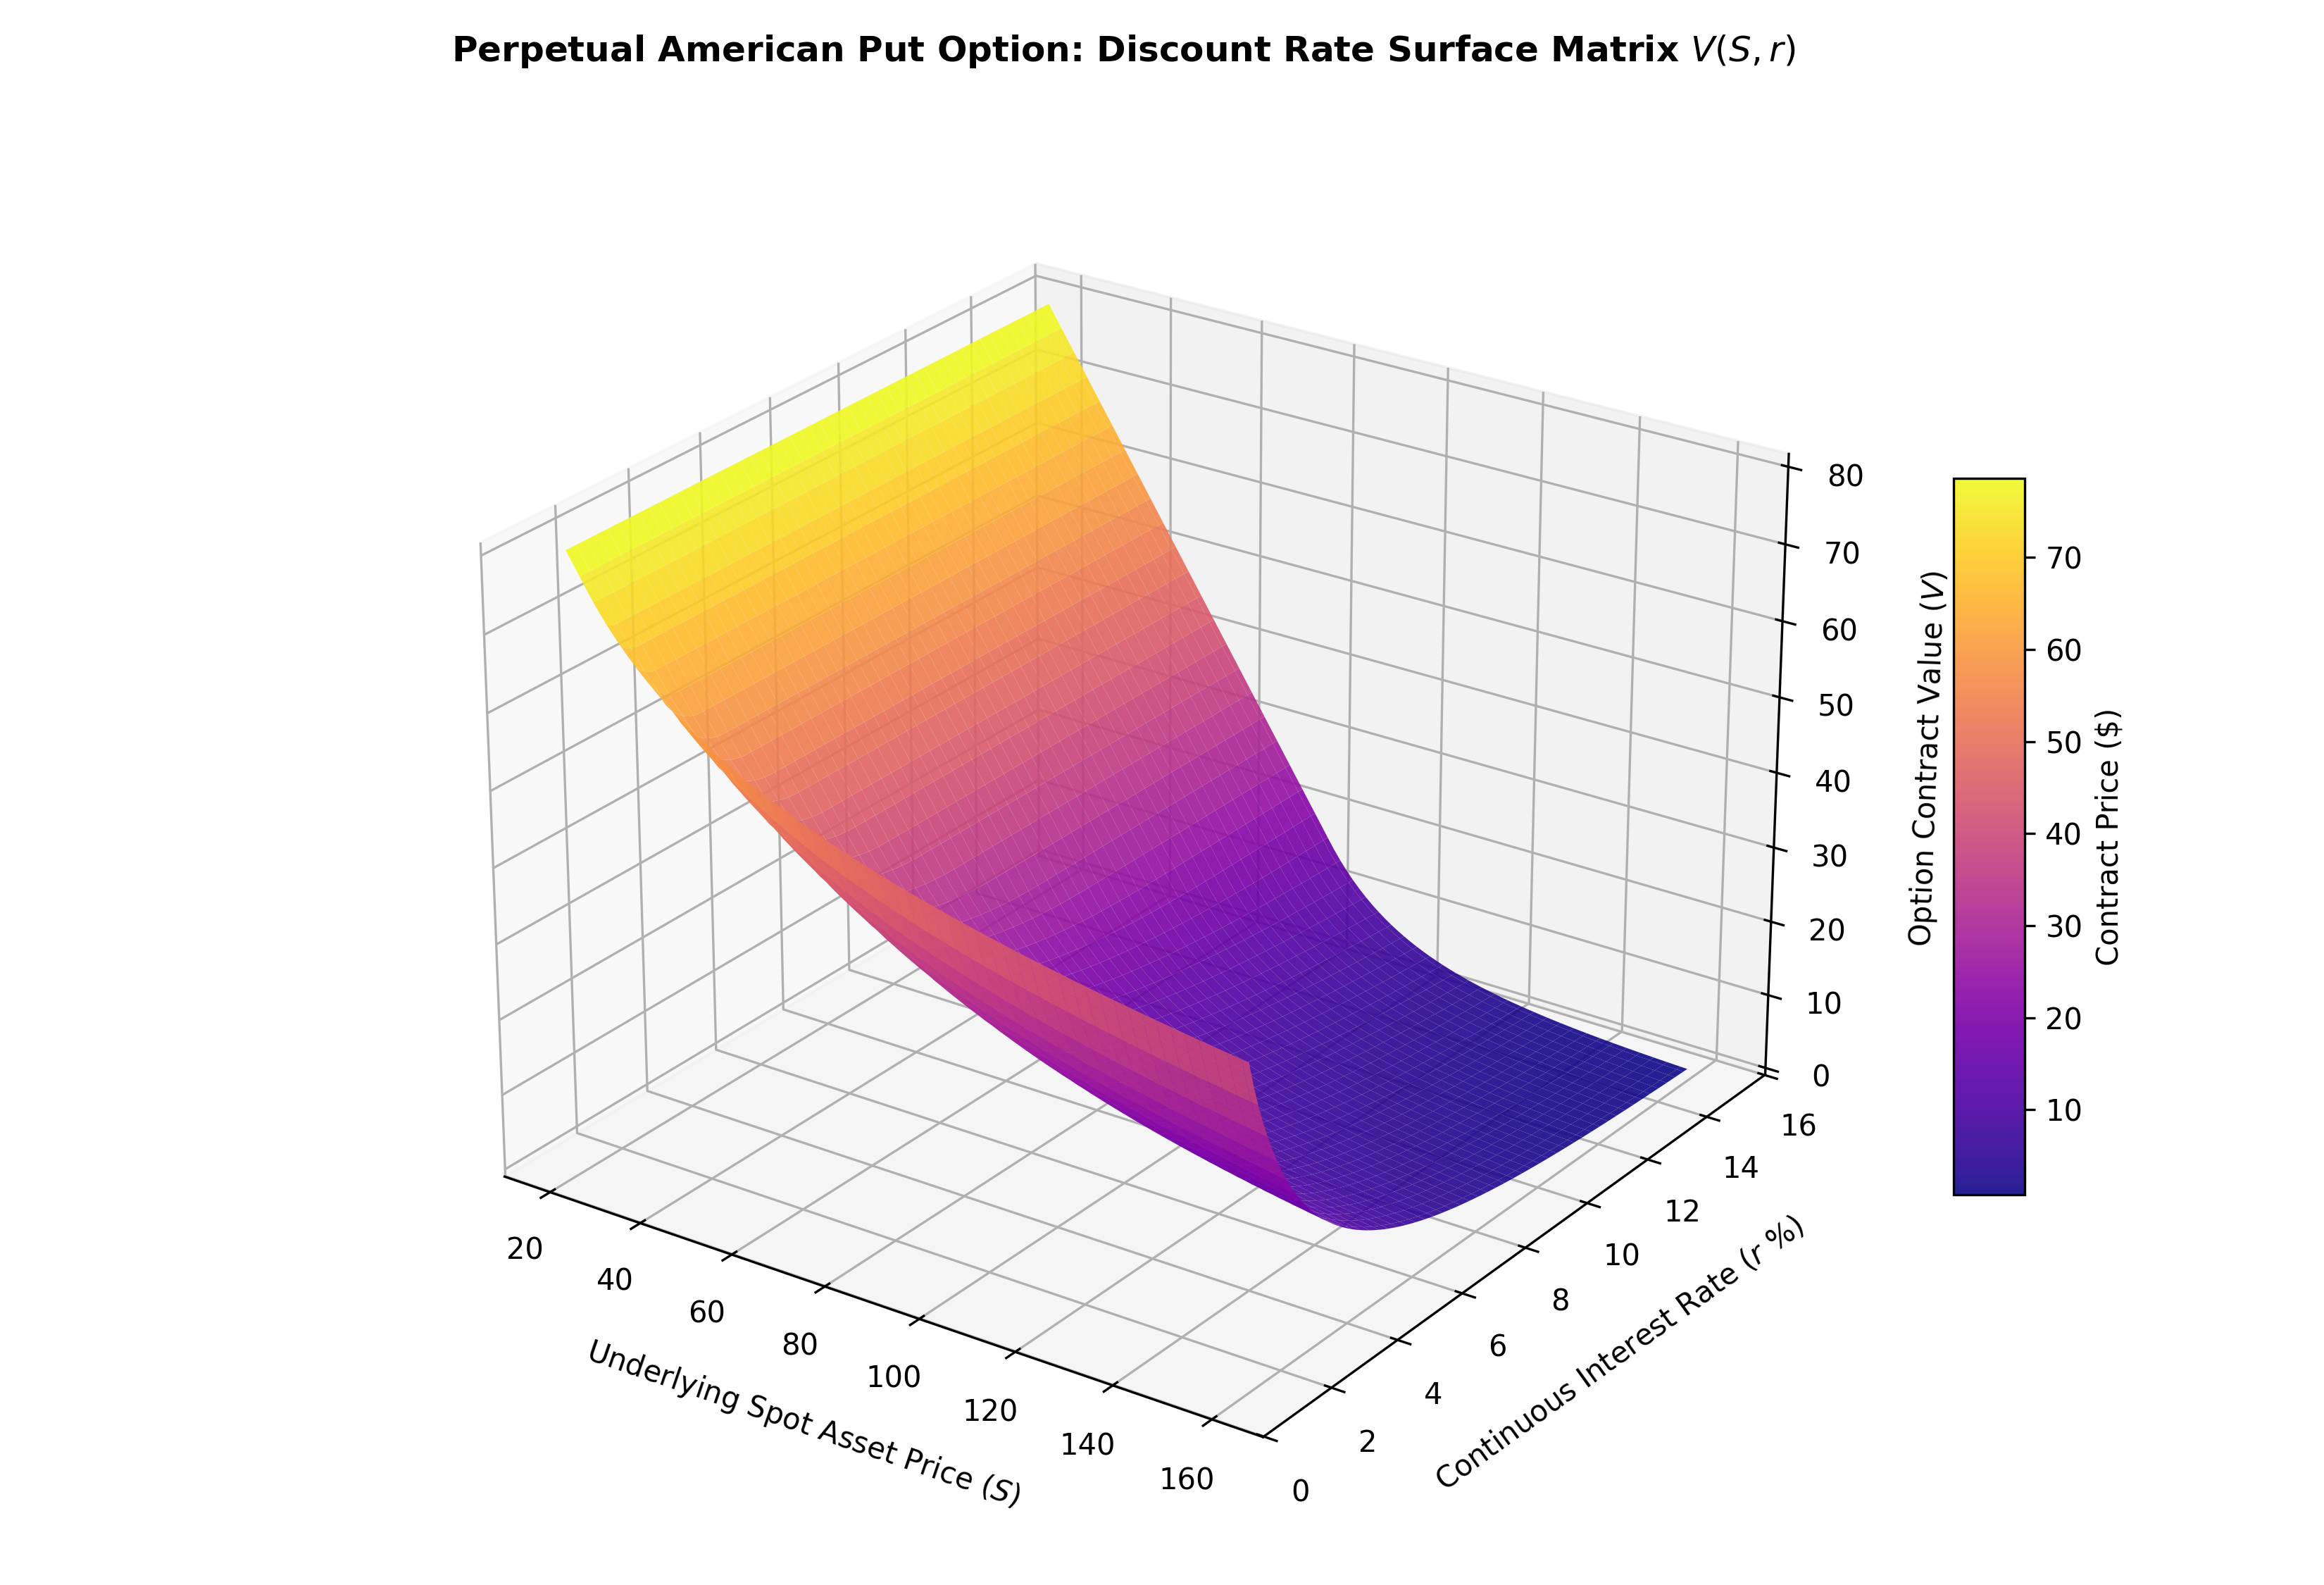
\includegraphics[width=\linewidth]{interest_surface_3d.png}
    \caption{Continuous 3D Monetary Discount Surface $V(S, r)$.}
    \label{fig:rate_surface_3d}
  \end{minipage}
\end{figure}


Figure \ref{fig:vol_surface_3d} demonstrates that as volatility rises along the axis, the option value surface physically warps upward in a convex manner. Conversely, Figure \ref{fig:rate_surface_3d} maps the asset matrix against changing macroeconomic yields, displaying a severe downward compression slope as rates scale toward $15\%$.


% ==========================================
% SECTION 5: FINANCIAL INTERPRETATION & CONCLUSION
% ==========================================
\section{Financial Interpretation}
While Section 4 established the geometric and mathematical consistency of the ordinary differential equation, 
interpreting these computational outputs through a macroeconomic lens reveals the real-world utility and predictive power of the model. 

\subsection{Economic Meaning of Limits and Boundaries}
The asymptotic limit proofs analyzed through the computational engine directly reflect human investor psychology and rational market behavior. 
The mathematical collapse of the optimal early exercise boundary $S^*$ to $\$0.00$ as volatility approaches infinity ($\sigma \to \infty$) proves that in a highly chaotic market, 
the structural ``option to wait'' becomes infinitely valuable. 
An investor will rationally hold the contract indefinitely to capture potentially massive downward asset swings, 
choosing never to extinguish the time-value component prematurely. 

Conversely, 
the intense compression of the pricing surface observed under high interest rates ($r$) highlights the macroeconomic opportunity cost of capital. 
When $r$ is elevated, 
holding an in-the-money contract without exercising penalizes delayed payouts due to a punishing discount factor. 
Under these monetary regimes, 
investors are heavily incentivized to trigger early cash exercise at a much higher asset threshold $S^*$ 
to liquidate their positions and immediately reinvest their capital into risk-free government yields.

\subsection{Visualizing Option Greeks via Surface Curvature}
The three-dimensional topological matrices generated by the simulation engine provide a dynamic continuous map of the contract's risk sensitivities, 
universally known in quantitative finance as the ``Greeks'' \cite{black1973pricing, hull2012options}. 
The spatial velocity at which the option value surface decays against shifts in the underlying spot 
asset price mathematically characterizes the contract's Delta ($\Delta = \frac{\partial V}{\partial S}$) \cite{hull2012options}. 
Near the continuous moving boundary $S^*$, Delta converges exactly to $-1.00$, graphically validating the smooth-pasting condition and proving the total absence of immediate arbitrage along the boundary layer. 

As the asset price expands into the far-field zone, 
the surface flattens out asymptomatically toward zero. 
The convex acceleration or rate of change of this velocity represents the option's Gamma ($\Gamma = \frac{\partial^2 V}{\partial S^2}$), 
visually proving that the contract's structural sensitivity to spot price fluctuations diminishes exponentially as the asset moves deeply out-of-the-money. 

\subsection{Structural Limitations of the ODE Framework}
Despite its analytical elegance and mathematical tractability, 
collapsing the classic Black-Scholes partial differential equation (PDE) 
into a single-variable ordinary differential equation introduces necessary real-world constraints. 
The core assumption underlying this framework is that both the risk-free yield $r$ and the asset standard deviation $\sigma$ remain strictly constant through time, 
allowing the temporal decay component ($\frac{\partial V}{\partial t}$) to be zeroed out entirely. 

In actual financial markets, 
macroeconomic interest rates are dynamically manipulated by central banks in response to shifting inflationary pressures, 
and asset volatility clusters unpredictably during systemic market shocks. 
To deploy options pricing systems within highly realistic institutional environments, 
practitioners must relax these rigid stationarity constraints and implement advanced stochastic volatility frameworks (such as the Heston model) or numerical partial differential equation solvers, 
though the perpetual ODE remains an indispensable foundational benchmark for risk architecture verification.

% ==========================================
% SECTION 6: CONCLUSION
% ==========================================
\section{Conclusion}
This research project successfully executed the end-to-end development of a perpetual American put option pricing framework, 
seamlessly bridging analytical calculus with custom object-oriented software design. 
By exploiting the temporal stationarity of perpetual contracts, 
the underlying free-boundary Black-Scholes PDE was reduced to a variable-coefficient ordinary differential equation. 
Solving this system analytically yielded a closed-form piecewise pricing schedule bound tightly by an optimal early exercise threshold $S^*$ and verified via strict smooth-pasting and far-field boundary conditions.

To validate the structural integrity of this mathematical engine, 
a robust Python simulation suite was engineered, mapping both 2D parameter sweeps and continuous 3D pricing surfaces ($V(S, \sigma)$ and $V(S, r)$). 
The computational output perfectly mirrored the theoretical asymptotic limits: proving that extreme volatility drives early exercise behavior to zero, 
while rising macroeconomic interest rates pull the exercise boundary closer to the strike price. 
Ultimately, this integration of rigorous differential equations, 
rigorous limit proofs, and multi-dimensional visual profiles demonstrates how computational tools 
can effectively translate abstract financial economic theory into highly predictive, visual, and stable risk-management software engines.

\vfill\pagebreak


% ==========================================
REFERENCES
% ==========================================


\bibliography{refs}   
\bibliographystyle{alpha} 

\end{document}